\subsection{Model}\label{sec:cloud:virtualized_network_functions:model}

In this section we provide a model for a traditional \gls{GGSN} and discuss a model for a virtual \gls{GGSN} using \gls{NFV}.
In \gls{NFV} \cite{Nfv2013} static network middleboxes are replaced by commodity hardware.
The tasks solved by the original middleboxes are then solved by dedicated software.

\subsubsection*{Traditional GGSN}\label{sec:cloud:virtualized_network_functions:model:traditional_ggsn}
First, we give a model for a \emph{traditional} \gls{GGSN}, i.e. a static network component.
While we consider the \gls{GGSN} to be one fixed entity, it can in reality consist of multiple servers.
However, due to the fact that the \gls{GGSN} is purchased from a vendor as a middlebox, idle servers can be neither deactivated nor reused for other purposes.

\begin{figure}
  \centering
  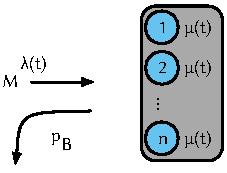
\includegraphics{cloud/virtualized_network_functions/model/figures/traditional_ggsn}
  \caption{Considered model of a traditional \headershortacr{GGSN}.}
  \label{sec:cloud:virtualized_network_functions:model:traditional_ggsn:model}
\end{figure}

We present an abstract queueing model for the traditional \gls{GGSN} in \reffig{sec:cloud:virtualized_network_functions:model:traditional_ggsn:model}.
New tunnels requests arrive according to a poisson process with rate \(\lambda(t)\) at the \gls{GGSN}.
This server will support a maximum tunnel capacity of \(c\).
When this capacity is reached, blocking will occur and newly incoming tunnels requests are rejected.
Traditionally, \glspl{GGSN} can be expected to be overdimensioned in such a way that this rarely happens.
If the new tunnel is accepted, it will occupy one of the serving units of the server for the duration \(\mu(t)\) of the tunnel.
As stated earlier, we can not model the tunnel duration to be markovian, resulting in a  \(M/GI/c\) loss system.
In order to give quality of service guarantees the network operator is interested in the system's blocking probability \(\blockingprobability\), which we consider to be a key metric of our model.
Additionally, the previously described diurnal patterns can are also be modelled by adjusting the arrival and serving process distributions for each time of day.
This alternatively also allows just to investigate the busy hour and thus the system's peak load.

\subsubsection*{\headershortacr{GGSN} using Network Function Virtualisation}\label{sec:cloud:virtualized_network_functions:model:virtual_ggsn}
Next, we introduce concepts from \gls{NFV}, i.e. the idea to replace middleboxes with commodity hardware as an extended model in \reffig{sec:cloud:virtualized_network_functions:model:virtual_ggsn:model}. 
This allows us to realise benefits from cloud computing, as we are now able to scale out, instead of up.
The assumptions of the Markov arrival process \(\lambda(t)\) and the serving time distributions \(\mu(t)\) are carried over.
However, instead of one server processing every tunnel, this model assumes that there are up to \(s_{max}\) virtualised servers \(s_i\).
Each of these is less powerful than the traditional \gls{GGSN}, having a tunnel serving capacity of \(c_i \ll c\) and a total system capacity of \(c_{max} = s_{max} \times i\).

\begin{figure}
  \centering
  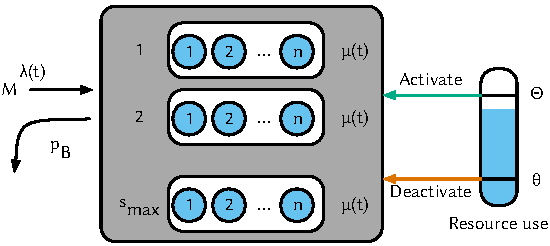
\includegraphics{cloud/virtualized_network_functions/model/figures/virtual_ggsn}
  \caption{Considered model of a virtualised \headershortacr{GGSN}.}
  \label{sec:cloud:virtualized_network_functions:model:virtual_ggsn:model}
\end{figure} 

In its initial state, for efficiency, all but a small portion of the server instances are considered to be disabled.
Only, when a certain condition is reached, a new server instance is provisioned.
As a simple example, one instance could be kept in reserve for upcoming requests and an additional would be provisioned as soon as the reserve is used.
Similar rules should apply in the shutdown of servers and form a hysteresis with the boot condition.
For example it would be possible to keep at least one server in reserve but never more than two.

If these conditions are not carefully selected and are in tune with the expected boot time of an instance, additional blocking can occur.
Despite not having reached its maximum capacity, this system would still reject tunnel requests during the provisioning phase when no tunnel slots are available.
This could be remedied by a request queue.
However, this would introduce additional complexity to the system without providing real benefit, as mobile devices or applications will repeat their attempts and would time out when the request is taking too long. 

To place incoming tunnel state on one of the available servers a load balancer is required. 
To ensure that the system in run time can scale down to its actual needs, the balancer should place tunnels on servers that are the fullest, keeping the reserve free.
It may even migrate tunnel state from almost empty servers away so that these can be shut down, when the shutdown condition is fulfilled.
Keeping instance close to their capacity should also have no impact on the performance a mobile device associated to a specific tunnel experiences.
